\tikzset{every picture/.style={line width=0.75pt}} %set default line width to 0.75pt        

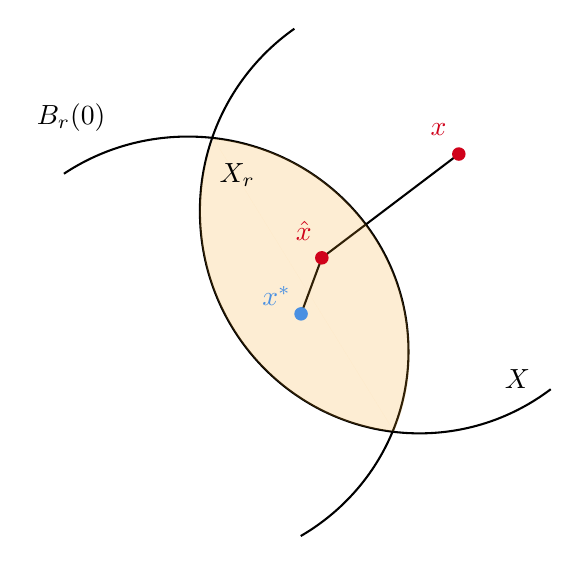
\begin{tikzpicture}[x=0.75pt,y=0.75pt,yscale=-1,xscale=1]
%uncomment if require: \path (0,269.33331298828125); %set diagram left start at 0, and has height of 269.33331298828125

%Straight Lines [id:da9081237263295667] 
\draw    (339.75,122.75) -- (405.75,72.75) ;


%Straight Lines [id:da013531378414466388] 
\draw    (329.75,149.75) -- (339.75,122.75) ;


%Shape: Arc [id:dp29762120971158423] 
\draw  [draw opacity=0] (450.04,186.06) .. controls (432.4,199.42) and (410.49,207.33) .. (386.75,207.33) .. controls (328.35,207.33) and (281,159.43) .. (281,100.33) .. controls (281,63.88) and (299.01,31.69) .. (326.52,12.37) -- (386.75,100.33) -- cycle ; \draw   (450.04,186.06) .. controls (432.4,199.42) and (410.49,207.33) .. (386.75,207.33) .. controls (328.35,207.33) and (281,159.43) .. (281,100.33) .. controls (281,63.88) and (299.01,31.69) .. (326.52,12.37) ;
%Shape: Arc [id:dp9736457048511031] 
\draw  [draw opacity=0] (215.51,82.23) .. controls (232.53,70.94) and (253.1,64.33) .. (275.25,64.33) .. controls (333.93,64.33) and (381.5,110.67) .. (381.5,167.83) .. controls (381.5,205.65) and (360.68,238.73) .. (329.59,256.79) -- (275.25,167.83) -- cycle ; \draw   (215.51,82.23) .. controls (232.53,70.94) and (253.1,64.33) .. (275.25,64.33) .. controls (333.93,64.33) and (381.5,110.67) .. (381.5,167.83) .. controls (381.5,205.65) and (360.68,238.73) .. (329.59,256.79) ;
%Curve Lines [id:da7464413291611462] 
\draw [color={rgb, 255:red, 0; green, 0; blue, 0 }  ,draw opacity=0 ][fill={rgb, 255:red, 245; green, 166; blue, 35 }  ,fill opacity=0.2 ]   (287.5,65.33) .. controls (262.5,132.33) and (312.5,201.33) .. (374.5,206.33) ;


%Curve Lines [id:da9820940956263626] 
\draw [color={rgb, 255:red, 0; green, 0; blue, 0 }  ,draw opacity=0 ][fill={rgb, 255:red, 245; green, 166; blue, 35 }  ,fill opacity=0.2 ]   (287.5,65.33) .. controls (360.5,72.33) and (399.5,149.33) .. (374.5,206.33) ;



%Shape: Circle [id:dp43139799952926605] 
\draw  [color={rgb, 255:red, 208; green, 2; blue, 27 }  ,draw opacity=1 ][fill={rgb, 255:red, 208; green, 2; blue, 27 }  ,fill opacity=1 ] (337,122.75) .. controls (337,121.23) and (338.23,120) .. (339.75,120) .. controls (341.27,120) and (342.5,121.23) .. (342.5,122.75) .. controls (342.5,124.27) and (341.27,125.5) .. (339.75,125.5) .. controls (338.23,125.5) and (337,124.27) .. (337,122.75) -- cycle ;
%Shape: Circle [id:dp14058981705181228] 
\draw  [color={rgb, 255:red, 208; green, 2; blue, 27 }  ,draw opacity=1 ][fill={rgb, 255:red, 208; green, 2; blue, 27 }  ,fill opacity=1 ] (403,72.75) .. controls (403,71.23) and (404.23,70) .. (405.75,70) .. controls (407.27,70) and (408.5,71.23) .. (408.5,72.75) .. controls (408.5,74.27) and (407.27,75.5) .. (405.75,75.5) .. controls (404.23,75.5) and (403,74.27) .. (403,72.75) -- cycle ;
%Shape: Circle [id:dp5811537747008597] 
\draw  [color={rgb, 255:red, 74; green, 144; blue, 226 }  ,draw opacity=1 ][fill={rgb, 255:red, 74; green, 144; blue, 226 }  ,fill opacity=1 ] (327,149.75) .. controls (327,148.23) and (328.23,147) .. (329.75,147) .. controls (331.27,147) and (332.5,148.23) .. (332.5,149.75) .. controls (332.5,151.27) and (331.27,152.5) .. (329.75,152.5) .. controls (328.23,152.5) and (327,151.27) .. (327,149.75) -- cycle ;


% Text Node
\draw (434,181) node   {$X$};
% Text Node
\draw (219,55) node   {$B_{r}( 0)$};
% Text Node
\draw (299,83) node   {$X_{r}$};
% Text Node
\draw (396,61) node [color={rgb, 255:red, 208; green, 2; blue, 27 }  ,opacity=1 ]  {$x$};
% Text Node
\draw (331,110) node [color={rgb, 255:red, 208; green, 2; blue, 27 }  ,opacity=1 ]  {$\hat{x}$};
% Text Node
\draw (318,141) node [color={rgb, 255:red, 74; green, 144; blue, 226 }  ,opacity=1 ]  {$x^{*}$};
\end{tikzpicture}
